% Chapte 8 
\chapter{Interactive and non-Interactive onsite study} % Main chapter title

\label{Chapter8} % For referencing the chapter elsewhere, use \ref{Chapter1} 

\section{Introduction}




The onsite study was executed in Weimar tourist Information Center at (Weimar Markt 10) which is one of important location for many tourists who visit Weimar. This location was chosen by Bauhaus-Spaziergang program personals that are providing tours for new visitors in Weimar. Bauhaus-Spaziergang does advertisement as brochure at this location. The location was reserved for our new advertisement starting from 1st February for three weeks. 

Two different Interactions and one non-Interactive Advertisement were made. The first one was body interaction where passerby can interact using his/her own body movement in the physical space and influence advertisement element in the screen. The second was mobile interaction where users by opening the advertisement web application in their smartphone can interact with advertisement and the third is a non-interactive advertisement where the interface and elements are completely similar but are not influence by people around, the elements change based on time-based random sequence. 



\section{Background}



\section{Interactive Advertisement}

The interactive advertisement was originally designed as a three distinctive phases.


\begin{enumerate}

\item \textbf{Attraction / Motivation phases:}\\ 
This phase is the first interface for the advertisement, the passerby silhouettes are being projected on the screen and in this interface Call-to-action is implemented to motivate passers-by to start interacting with the screen.
Call-to-action techniques were different for mobile and body interactive system.

\item \textbf{Interaction phase:} \\
This phase allows participants to actively influence the advertisement elements, which were highlighted regions of Bauhaus in Weimar, the participant could explore those regions just by reaching to them, a picture of the area with a short description would appear for three seconds and then fade out. This phase is constraint with time and will automatically be over with in 40 seconds and would switch to the last phase called ad video phase.

\item \textbf{Advertisement video phase:} \\
This phase only shows a 20 second non-interactive Bauhaus-spaziergang Ad video and whenever the video is over it will switch back to the initial phase.

\end{enumerate}

\subsection{Body Interactive}

The body interactive advertisement has the ability to detect up to seven people at a time and project their silhouette in the screen each with different colors, the Call-to-Action feature asks viewers to come near to the screen to start the interaction, when the interaction starts participants are given a short instruction on how to play the system, participants should walk physically in front of the screen in order to move the silhouette on the map to explore the regions. The interaction finishes if all the regions are explored or the 40 second time gets over and the Ad video is shown.


\begin{figure}[H]
    \centering
    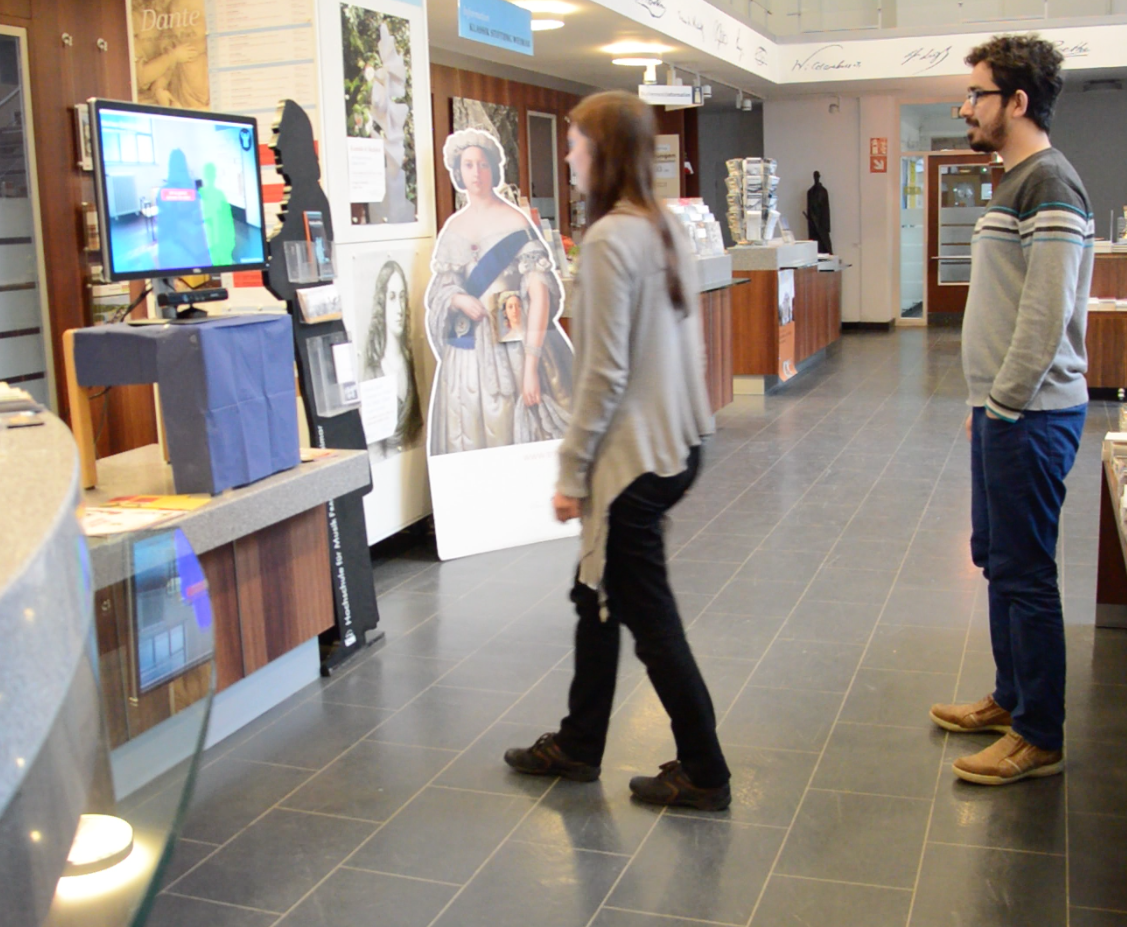
\includegraphics[width=110mm,height=70mm]{Figures/8/body_motivation}%
    \caption{Two persons are standing far from the screen, and their colored silhouettes are shown, the girl is getting closer to the screen to start the interaction.}%
    \label{fig:bodymotivationsystem}%
\end{figure}

\begin{figure}[H]
    \centering
    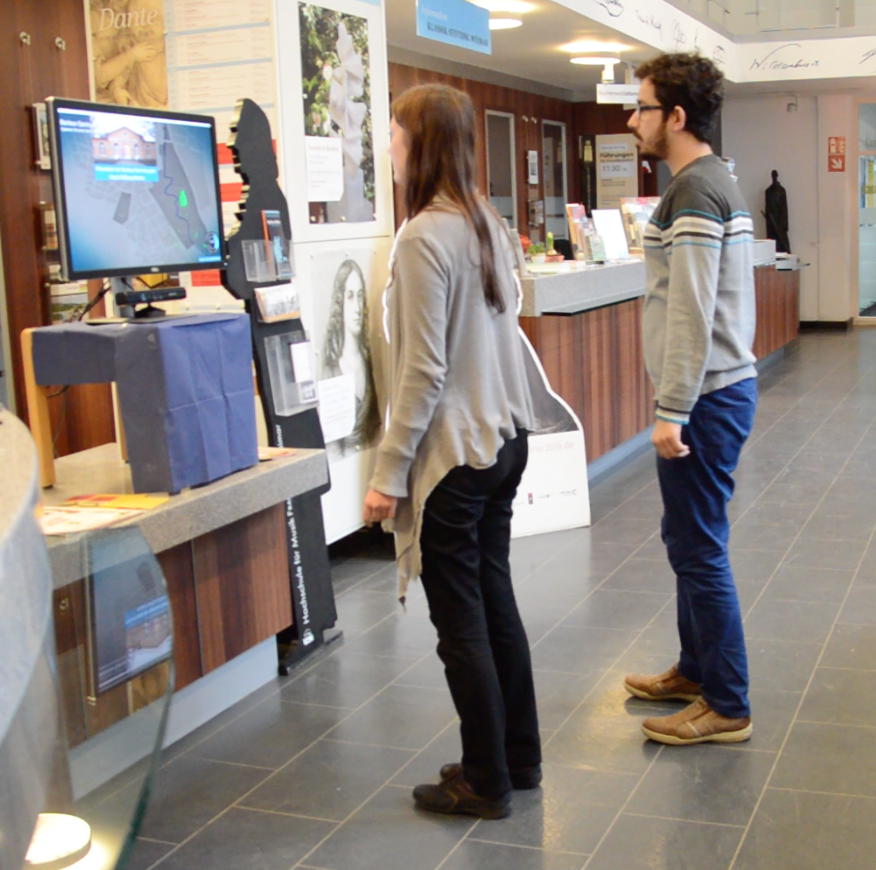
\includegraphics[width=110mm,height=70mm]{Figures/8/body_interaction}%
    \caption{Both are in interaction phase, as you can see the girl has explored one location and a picture is shown}%
    \label{fig:bodyinteractionsystem}%
\end{figure}

\subsection{Mobile Interactive}
As you already got the idea that this technique works with smart phone, the system also shows partially passers-by silhouette for attracting attention, but the Call-to-Action is done through using a mobile phone, the screen gives instruction on how to access the system. Passerby should connect to the wireless local area network and browse the controller website from their phone, and the control opens in their phone to use navigate to different regions on the map to explore interest locations. The interaction is also constraint to 40 second time and after that the Ad video is shown.


\begin{figure}[H]
    \centering
    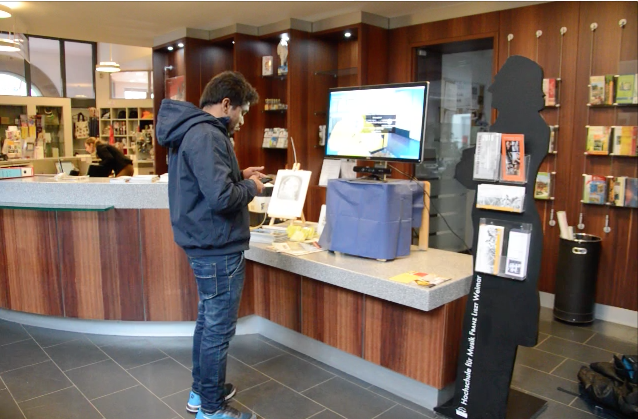
\includegraphics[width=110mm,height=70mm]{Figures/8/mobile_motivation}%
    \caption{The person is connecting to the advertisement web controller using his phone.}%
    \label{fig:mobilemotivationsystem}%
\end{figure}


\section{Non-Interactive Advertisement}
This technique is also composed of the same three phases but each of them is triggered without the influence of people around, we call it auto active advertisement too. The first phase shows only the screen with the Bauhaus-spaziergang title and has no Call-to-Action feature and after few seconds switches to the second phase, in second phase the locations are automatically explored in random sequence each time and has the same expiration time (40 seconds) as others and after that the same ad video is shown and switches back to the first mode. The entire cycle of the phases is around 60 seconds which is almost similar to the other two interactive advertisement.


\begin{figure}[H]
    \centering
    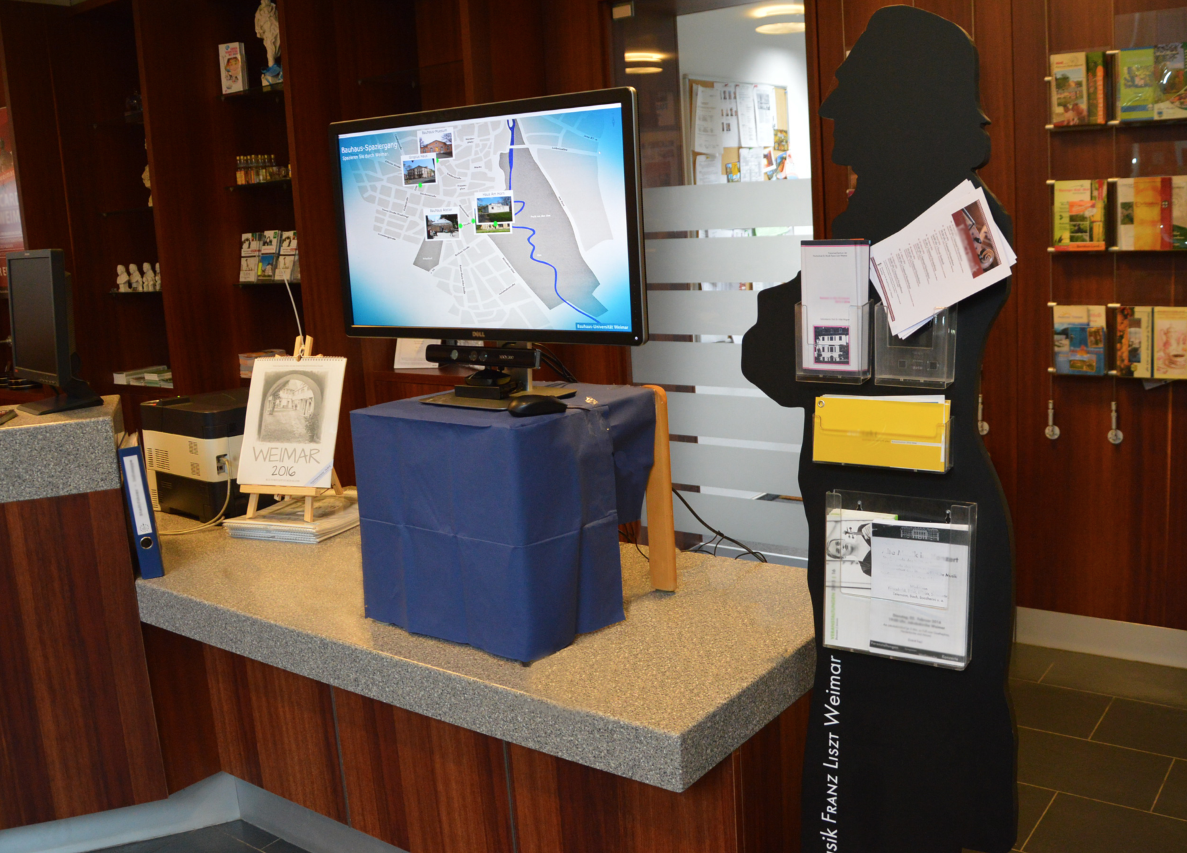
\includegraphics[width=110mm,height=70mm]{Figures/8/non_inter_screen}%
    \caption{The screen is automatically exploring locations on the map}%
    \label{fig:non-inteactivescreen}%
\end{figure}



\section{Problem Statement}
\begin{enumerate}

\item	For which of the three conditions (body, mobile and non-interactive advertisements) passers-by 

\begin{enumerate}
\item	Are more attracted toward.
\item	Perform Honeypot and Landing effects.
\item	Are engaged with the screen.
\item	Spend extra time for watching the remaining advertisement video after interaction.
\end{enumerate}

\item	How many people understand advertisement?
\item	Get general opinion about the advertisement techniques.
\item	Comparison of the techniques in between.

\end{enumerate}




\section{Design study}


\subsection{Location}
The screen was installed in Weimar Tourist Information center. This center is one of the famouse tourist information in Weimar where alot of tourists visit. Most importantly this location was chosen because our target audience (tourists) mainly elders visit.

\begin{figure}[H]
    \centering
    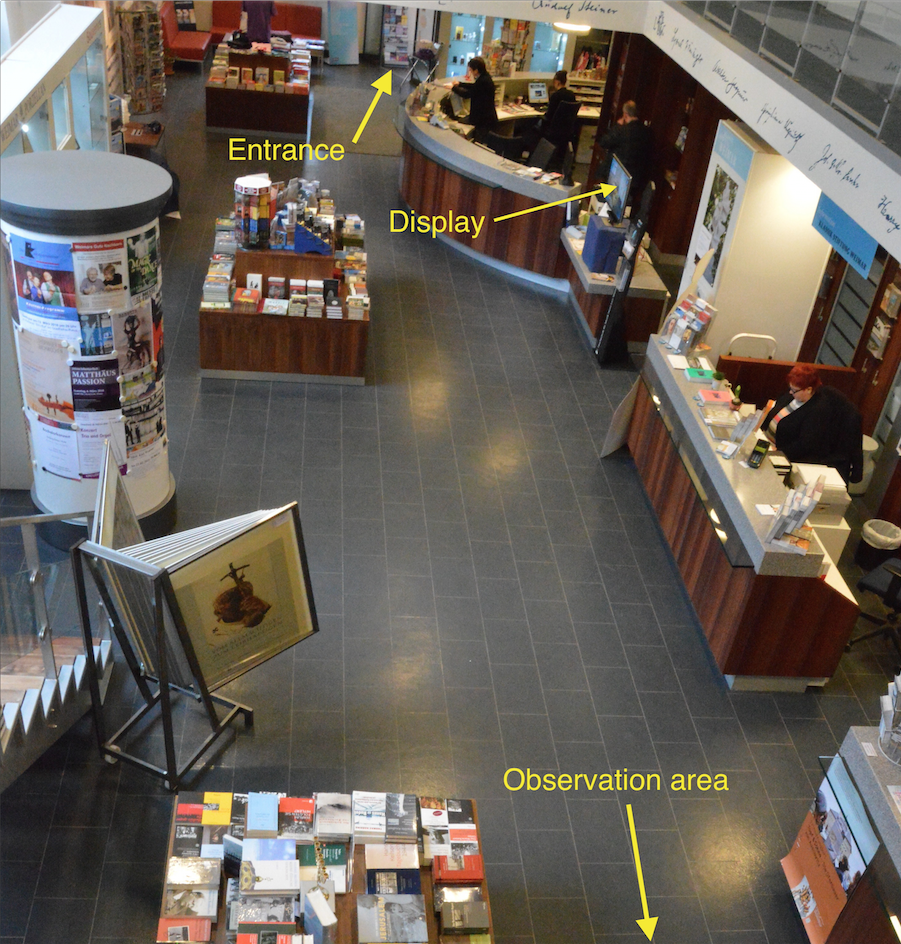
\includegraphics[width=110mm,height=90mm]{Figures/8/tourist_info}%
    \caption{Weimar Tourist Information Center Top-view picture, The locations are marked with yellow arrows.}%
    \label{fig:Tourist_info_center}%
\end{figure}


\subsection{Duration}
Each type of advertisement technique were installed for five days in the following three weeks.

\begin{table}[H]
\caption{Week sequence}
\label{tab:advertisementWeeks}
\centering
\begin{tabular}{l c c c }
\toprule
\tabhead{Advertisement} & \tabhead{1st Week} & \tabhead{2nd Week} & \tabhead{ 3rd Week} \\
\midrule
\textbf{Non-Interactive}     &   X    &         &     \\
\textbf{Body Interactive}     &        &    X    &    \\
\textbf{Mobile Interactive}  &        &         &   X   \\
\bottomrule\\
\end{tabular}
\end{table}



\subsection{Internal Validity}
To be confident that the change in the weeks would not effect the findings, 
Extra effort was done to make all the week environmental conditions the same as much as possible. The screen was installed in the same location, had the same screen brightness, height and also the surroundings of the screen were not altered, we asked the responsible person in tourist information center not to change anything in the surrounding. The luck was also with us that almost the weather conditions were the same too,but the only thing we could not change was the number of passerby; The flow of passerby should also be nearly the same.


\subsection{Participants}
The participants were the ones who pass by the screen, none of the participants were informed about this study nor any notes were put at the entrance. Roughly \%60 of the participants were elder aged between 30-60, \%25 were young and the rest \%15 were children.


\subsection{Data gathering}
Several types of data from different aspects were gathered for each individual week to be able for analyzing and also be able to answer new arising questions after the onsite evaluation, the bellow types of data were gathered.


\begin{enumerate}
\item \textbf{On-Site Observation} \\
Observation periods were arranged in two different time slots per day, the first time slot was from 10:00 – 12:00 and the second was from 14:00 – 16:00, except for Saturday and Sunday where the tourist information center was open only until 14:00, then the observation period was from 10:00-12:00 and 13:00-14:00. During these two time slots the bellow observations were made and to remove the effects of specific time order,the orders were counterbalanced.

\begin{enumerate}
\item \textbf{Attention Level measurement} \\
Attention level is how much a person gives attention to the display, which consist of number of glances and number of ignores and how much long a person is standing infront of the display.At the beginning gaze-tracking method was considered for accurate measurement of attention level, a very impressive work have been done from Intraface \cite{Intraface} that can not only detect glances but also human emotions at the time, but because of high flow rate that method was not used and instead the glance counting which was proposed by \cite{glancingcount} that has formalized a ranking system from which  glance is considered if a person reacts to the display by turning his/her head toward it that last less than 3 seconds.

One hour attention level counting for each time slot was conducted, in which the observer was writing the number of people passing by and how many of them glanced and ignored the screen.see the glance counting sheet in Appendix: \ref{AppendixA}.1

\item \textbf{Passerby behavior and Interviews} \\
During one hour per time slot per day the passerby behavior were observed like how they approach to the screen, how do they react, what path the passerby take and what are they looking for and even how they ignore the display and after they are done with the screen engagement a very short interview was taken from them. 

\end{enumerate}


\item \textbf{System Logs} \\
The Advertisement application can generate the bellow logs.
\begin{enumerate}

\item	\textbf{Non-Interaction application} \\
Only duration(seconds) spent in front of the display is logged for each individual person.

\item	\textbf{Interaction application}\\
For this type the system can detect

\begin{itemize}
\item	Time user joins.
\item	Interaction completion time.
\item	Number of tasks (locations) explored.
\item	Whole duration spent(sec).
\item	If the user has seen advertisement or not.
\end{itemize}

\end{enumerate}

\item \textbf{Interviews} \\
Interviews were taken from the passerby that had some sort of engagement with the display like for non-interactive advertisement the people were interviewed that they stood for a while and saw the advertisement and for the interactive advertisement the people were interviewed that interacted or tried to interact with the system.
A leaflet, that describes the thesis goal and interview consent form was handed to the participants and after signature the interview was conducted. All the interviews were audio recorded and later transcribed for analysis, all interviews took in average 4 minutes, the reason we took short interviews was that most of the people were tourists and had little time to stay and even some of them rejected interview because of shortage of time.
Each week there were some variation in the questions dependent to the type of advertisement.  See appendix \ref{AppendixD}.1


\item \textbf{Colored-image recording} \\
Colored-image recording from Kinect camera was done during entire three weeks for non-interactive and interactive advertisement for many reasons.

\begin{itemize}
\item Match the log data with the video data for accuracy.
\item Measure the number of Honeypot effects and landing effects.
\item Observe passerby behavior in detail.
\end{itemize}

Because of limited space and processing power, the actual depth information (x,y,z) for individual points was not stored but a 2D colored image was taken per second and after the image recording was done, in lab another post processing script was applied to integrate a static background using Adobe Photoshop application. To match the data logs and the image frames each image name consisted the date and time as (10.12.43.21.png).

\begin{figure}[!htb]
    \centering
    \subfloat[]{{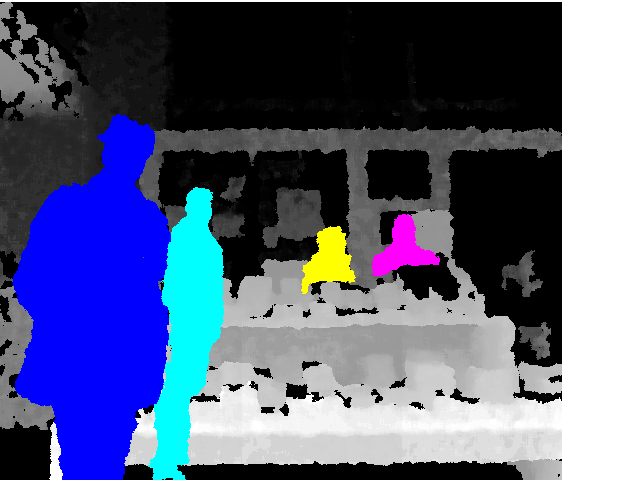
\includegraphics[width=50mm,height=40mm]{Figures/8/d1} }}%
    \subfloat[]{{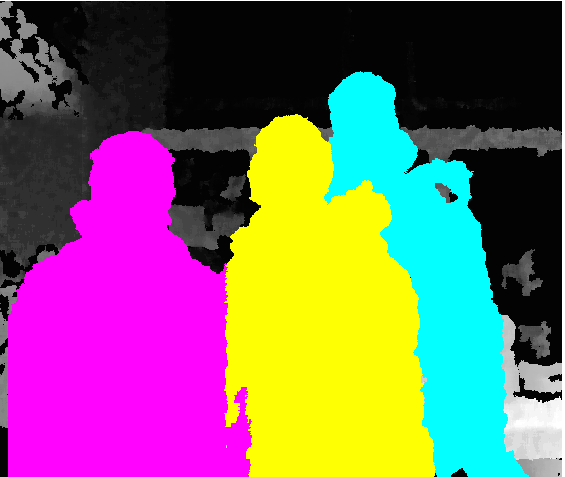
\includegraphics[width=50mm,height=40mm]{Figures/8/d2} }}%
    \caption{Depth recording examples}%
    \label{fig:DepthRecordedImages}%
\end{figure}

\end{enumerate}

Other pictures were also taken using mobile phone from the scene, verbal permission were taken before the photographing them.


\newpage
\section{Data Analysing}

 
\subsection {Glance counts} 
The glance counts were transformed from paper to spreadsheet in which number of glances and ignores were recorded individually and then combined from which mean value and percentages are extracted. see Appendix \ref{AppendixD}.2, \ref{AppendixD}.3 and \ref{AppendixD}.4 for each week.

\subsection {Interviews} 
All the interviews were transcribed and color coded from which interesting categories had emerged, each code is separately discussed in the finding section, To see color coded diagram see Appendix \ref{AppendixD}.5, \ref{AppendixD}.6 and \ref{AppendixD}.7 for each week


\subsection {Display Engagement phases and time} 
Log files along depth images were seen and compared to have accurate values for each engagement phases and the whole interaction phases. depth frames were manually frame-by-frame analysed and the logs were cleared from any possible mistakes.

\subsection {Honeypot and landing effects}
These two effects were observed mainly from the depth frames and also partially from onsite observation.

\subsection {Other observations}
The observations were done onsite, the observer wrote down any important event happened at that moment, These notes also include observer own point of view of understanding the scenario during the entire day and week. Most of the notes have time stamp. See Appendix \ref{AppendixD}.8, \ref{AppendixD}.9, and \ref{AppendixD}.11.\\
The depth recordings were also observed frame-by-frame to see anything that was missed when the observer was not present at the center. Different behaviors are extracted from the observation, which you will find in findings.



\newpage
\section{Findings}



\subsection{Individual advertisement}


\subsubsection{Non-Interactive findings}



\begin{enumerate}

\item Attention Level measurements

\begin{figure}[H]
    \centering
    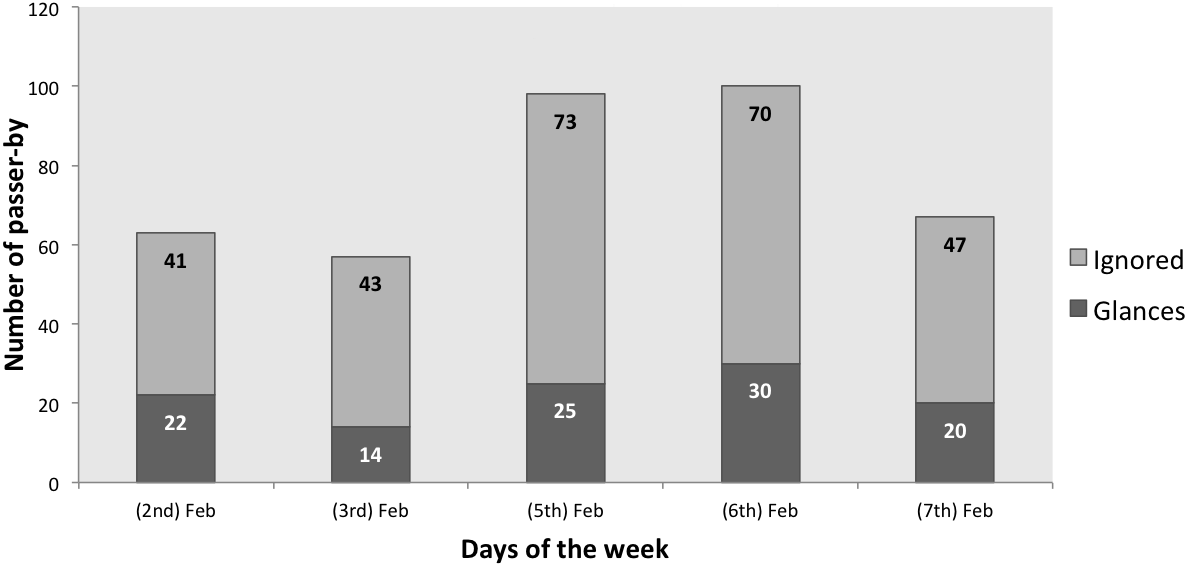
\includegraphics[width=110mm,height=55mm]{Figures/8/non_inter_findings/Non_Inter_chart}%
    \caption{Non-interactive attention level chart}%
    \label{fig:Nonattentionlevelchart}%
\end{figure}



\begin{figure}[H]
    \centering
    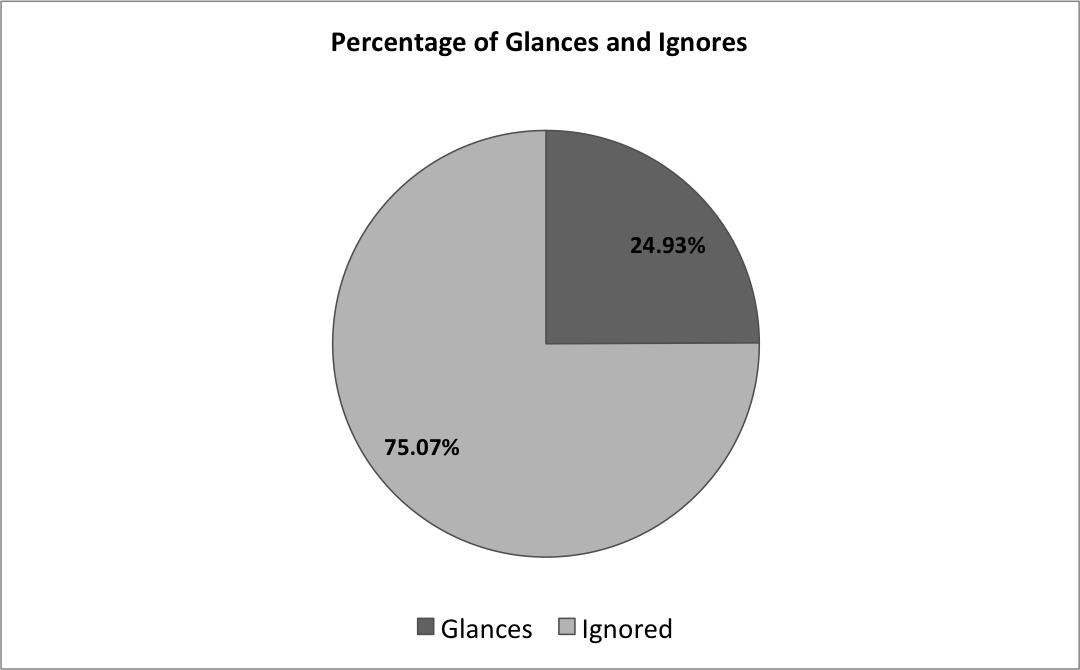
\includegraphics[width=110mm,height=55mm]{Figures/8/non_inter_findings/non_inter_percentage}
    \caption{Non-interactive Attention level percentage}%
    \label{fig:Nonattentionlevelpercentage}%
\end{figure}



\item Engagement time
The average engagement time was about 34.02 seconds.

\item Passerby and engagement


\begin{figure}[H]
    \centering
    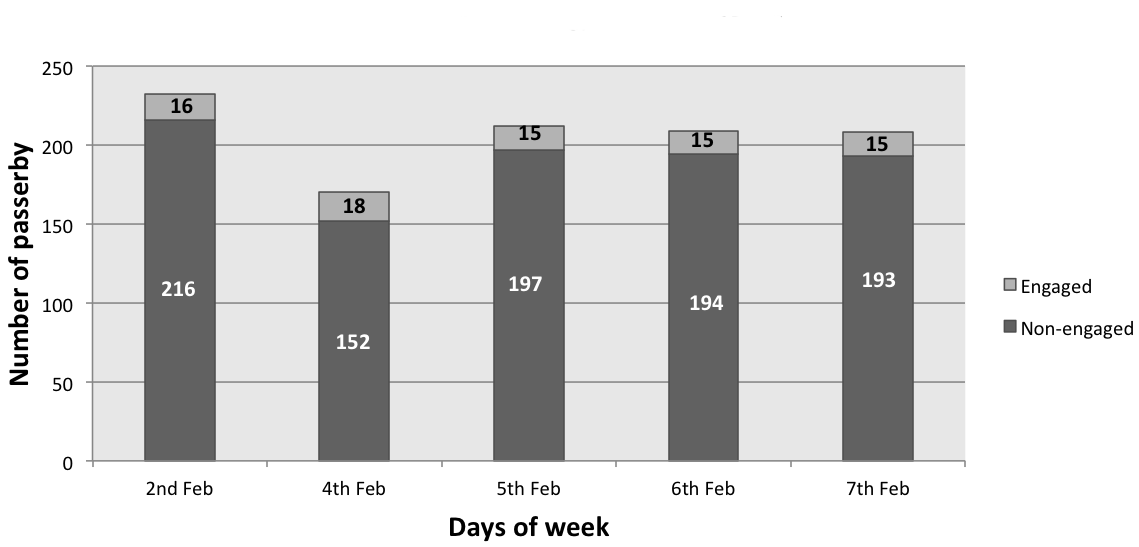
\includegraphics[width=110mm,height=60mm]{Figures/8/non_inter_findings/non_inter_engage_day}
    \caption{Non-interaction Number of engaged passerby}%
    \label{fig:Nonengagedandengagedby}%
\end{figure}

\begin{figure}[H]
    \centering
    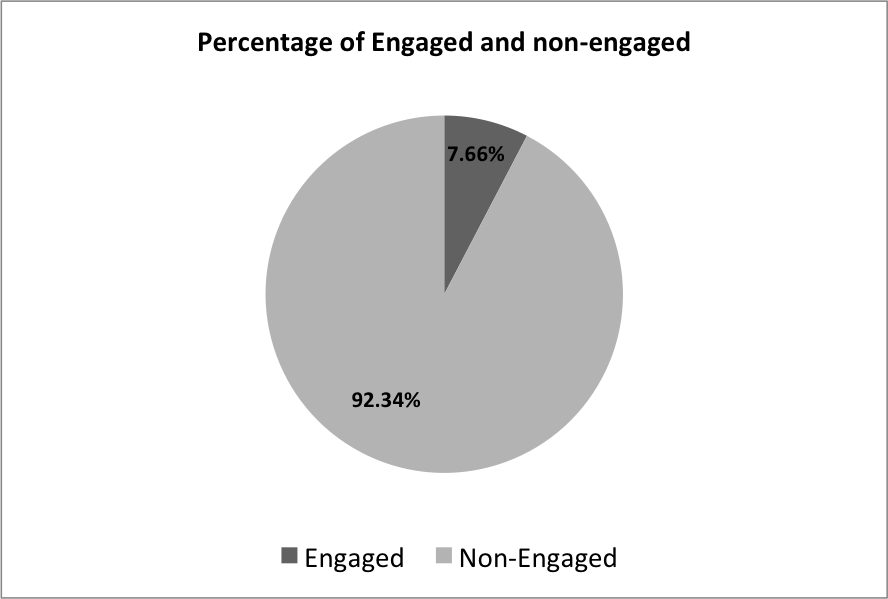
\includegraphics[width=110mm,height=60mm]{Figures/8/non_inter_findings/non_eng_percentage}
    \caption{Non-Interactive Percentage of engaged and passerby}%
    \label{fig:Nonengagedpasserbypercentage}%
\end{figure}


\item Landing and Honeypot effects

\begin{table}[H]
\caption{Landing and honeypot effects}
\label{tab:landingandhonypot}
\centering
\begin{tabular}{| l | c | c |}
\toprule
\tabhead{Days} & \tabhead{Landing effect} & \tabhead{Honeypot effect} \\
\midrule
\textbf{2nd Feb}  & 1 &  1 \\
\textbf{4th Feb}  & 0 &  1 \\
\textbf{5th Feb}  & 2 &  3 \\
\textbf{6th Feb}  & 0 &  3 \\
\textbf{7th Feb}  & 1 &  1 \\
\bottomrule
\end{tabular}
\end{table}

\item Interview

\begin{enumerate}

\item Likes \\
Many things from the advertisement were interesting, like the concept of map and the design. As one stated that, ``\emph{I find the idea good, it is nice to see the pictures of the places on the map}'', ``\emph{it is very nice idea because it will be remembered and when I go to the city I will remember}''

\item Dislikes \\
Most of the respondents complained on the speed of the advertisement that how fast the image changes as one said ``\emph{But the pictures were changing very fast}'' other said, ``\emph{advertisement is a little fast}'' They mentioned that why speed is an issue as stating, ``\emph{we wanted to see the map}'', ``\emph{ Could not read the text}''. Many things were disliked by some of the respondents like the advertisement theme, one said, ``\emph{It did not have Bauhaus Theme, the color and that design}'' One respondent also disliked the blinking points.

\item  Participation \\
Respondents mentioned the same excuses that were given at body interactive advertisement, one said, ``\emph{I will join if I am free}'', other said, ``\emph{I have no time}'', or ``\emph{if the weather is good}''. 

\item  Advertisement recall
People could recall the ad, as one mentioned, ``\emph{It is for a tour of Bauhaus in Weimar}'' other said, ``\emph{People can visit the city}'' and some mentioned directly the name of the program ``\emph{Bauhaus-Spaziergang}''.

\item Recommendations \\
There were many recommendations proposed by the responders, which was on content, speed, design.Content related recommendations was that one said, ``\emph{If the prices are mentioned it would be good so that they can decide if they want to take it or not}'' other said on timing, ``\emph{how long does this tour take so people arrange their}''. Another mentioned on speed like ``\emph{it must be little slow}''.

\end{enumerate}


\item Note taking


See appendix  \ref{AppendixD}.8


\item Other observations

Discuss on bellow things

Approaching to the screen

describe the other pictures you have saved in the folder


\end{enumerate}


\subsubsection{Body Interactive findings}

\begin{enumerate}
\item Attention Level measurements


\begin{figure}[H]
    \centering
    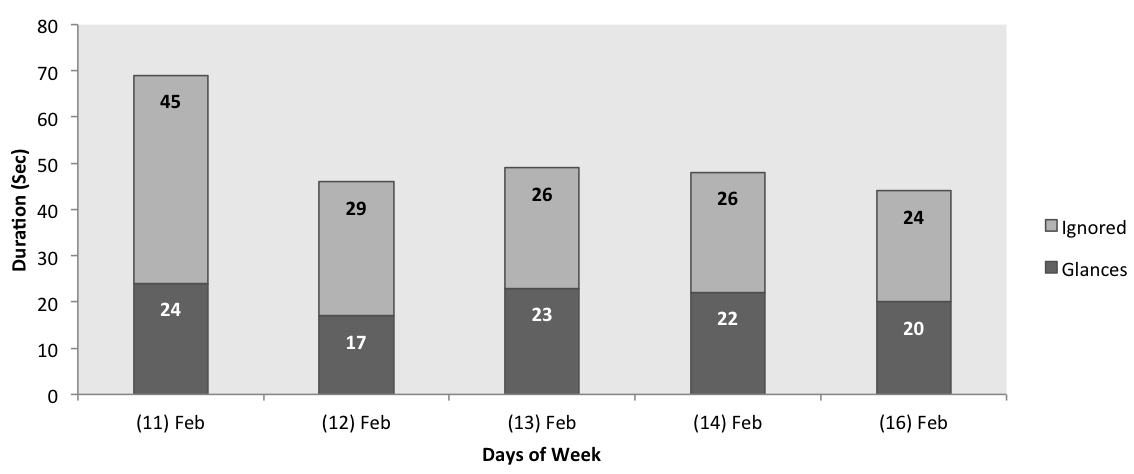
\includegraphics[width=110mm,height=60mm]{Figures/8/body_inter_findings/Body_Inter_chart}%
    \caption{Body interactive attention level chart}%
    \label{fig:bodyattentionlevelchart}%
\end{figure}


\begin{figure}[H]
    \centering
    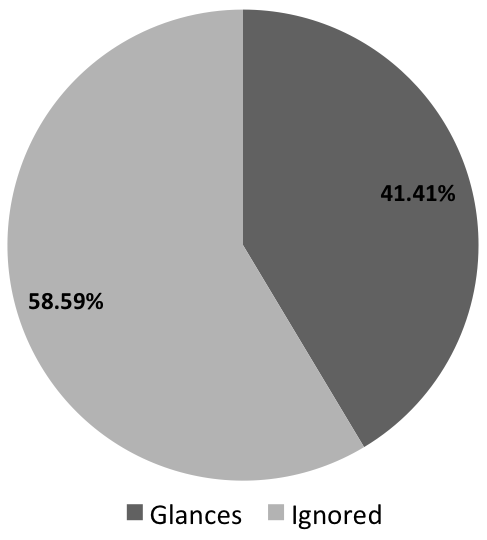
\includegraphics[width=110mm,height=60mm]{Figures/8/body_inter_findings/body_inter_percentage}
    \caption{Body interactive Attention level percentage}%
    \label{fig:bodyattentionlevelpercentage}%
\end{figure}



\item Engagement time

41.84 sec are spent in average



\item Engagement phases

\begin{figure}[H]
    \centering
    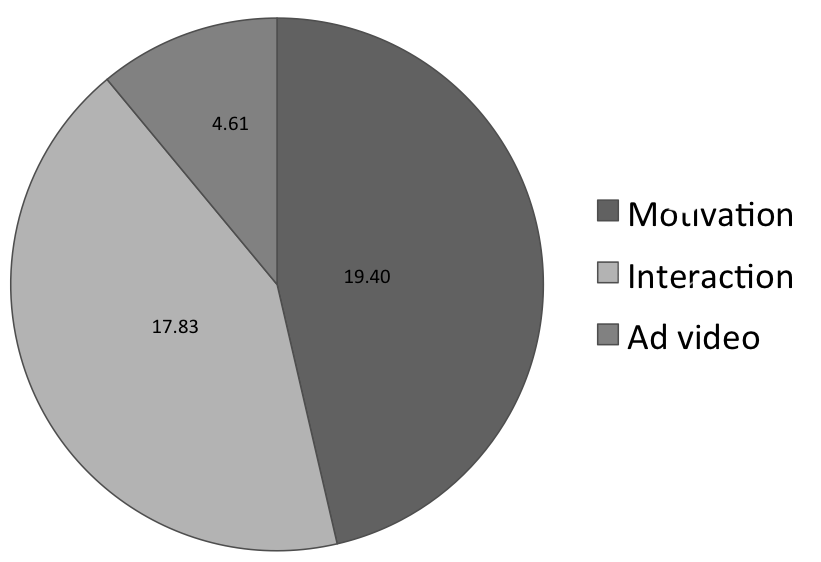
\includegraphics[width=110mm,height=60mm]{Figures/8/body_inter_findings/body_avg_phases}
    \caption{Average time for each phase}%
    \label{fig:bodyaveragephases}%
\end{figure}



\item Passerby and interactions

\begin{figure}[H]
    \centering
    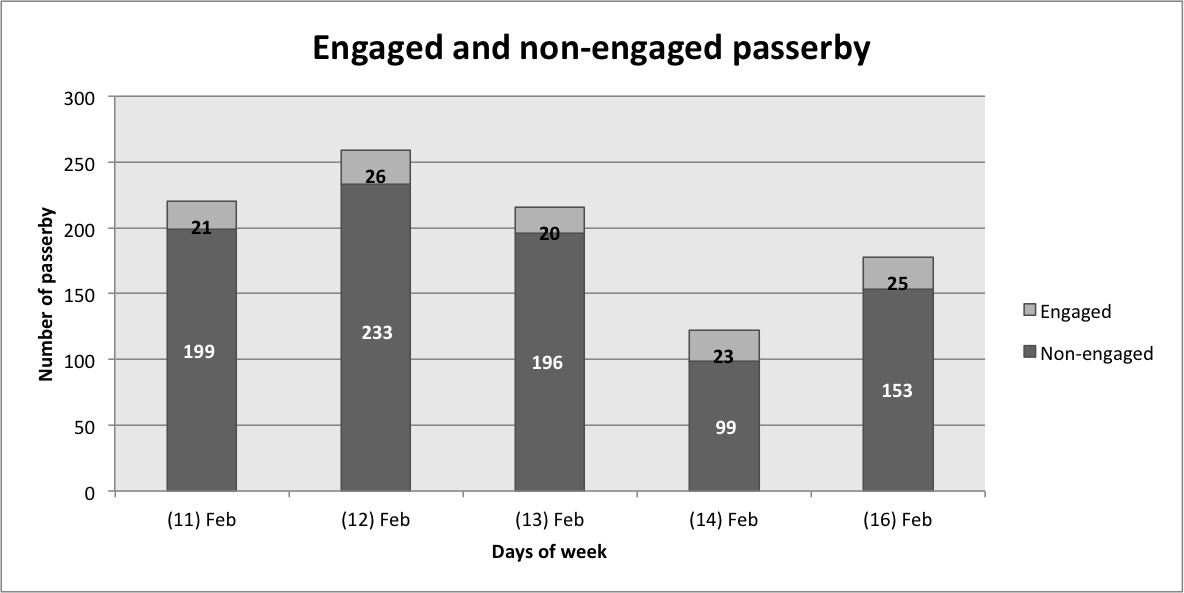
\includegraphics[width=110mm,height=60mm]{Figures/8/body_inter_findings/body_inter_engage_day}
    \caption{Body interactive Number of engaged passerby}%
    \label{fig:bodyengagedandengagedby}%
\end{figure}

\begin{figure}[H]
    \centering
    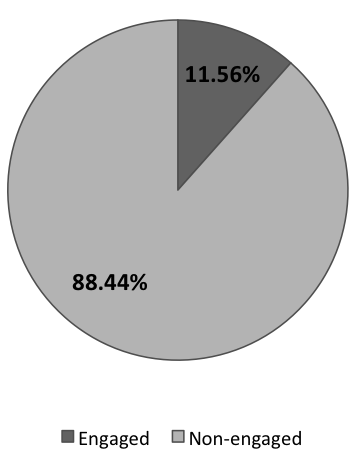
\includegraphics[width=110mm,height=60mm]{Figures/8/body_inter_findings/body_eng_percentage}
    \caption{body interactive percentage of engaged passerby}%
    \label{fig:bodyengagedpasserbypercentage}%
\end{figure}


\item Landing and Honeypot effects

\begin{table}[H]
\caption{Body Interactive Landing and honeypot effect}
\label{tab:landingandhonypot_body}
\centering
\begin{tabular}{| l | c | c |}
\toprule
\tabhead{Days} & \tabhead{Landing effect} & \tabhead{Honeypot effect} \\
\midrule
\textbf{11 Feb}  & 2 &  2 \\
\textbf{12 Feb}  & 3 &  3 \\
\textbf{13 Feb}  & 2 &  2 \\
\textbf{14 Feb}  & 2 &  5 \\
\textbf{16 Feb}  & 3 &  3 \\
\bottomrule
\end{tabular}
\end{table}


\item Interview


The interviews were coded each individually and as a result the bellow categories are extracted, these categories are mainly taken from the questions and others are from the replies of the participants. 

\begin{enumerate}

\item Noticing \\
    Different people had their different experience and reaction when they noticed themselves in the display for the first time. Some of the people were standing and looking some books for long time when they saw themselves and for confirmation they waved toward the screen, as one said ``\emph{Yes at first I thought that it is not me. I waved my hand and came near.}'' Other said, ``\emph{Yes I saw my blue color body}''. Other participants noticed at the time of passing from front of the screen, ``\emph{when I was passing I saw myself in the screen.}'' Other people saw their friend first then noticed themselves like one said, ``\emph{I saw my friend in the screen and came near and I was also there with blue color.}'' One participant who usually comes to the center every week said that because the screen was newly installed I came near to the screen to see what is new inside.

\item Ad recall \\
    Respondents responded accurately the content and goal of the advertisement as one said, ``\emph{It was about a tour of Bauhaus, Bauhaus Spaziergang.}'' ``\emph{It was about tour in the city.}'' And other said, ``\emph{It was about Bauhaus-Walk. City tour.}'' And other said, ``\emph{it is something to do with Bauhaus city walk}''.

\item Interest \\
    People find this type of interaction very interesting, funny and motivative, one participant mentioned that, ``\emph{I liked to see myself in the screen, it was funny.}'' Other says the use of media is very interesting and comfortable for people, ``\emph{I think that the people with the use of media is comfortable}''. The use of this type of interactive advertisement give people some sort of good feeling toward Bauhaus-Walk event like one said, ``\emph{Bauhaus is very interested to me and it sounds fun}''. People also liked the way content was inside the advertisement like one said, ``\emph{It is very interesting to see the pictures}'' and even one participant exactly mentioned the goal of the advertisement interaction, ``\emph{it was a very interesting idea and it is like a small interactive tour for the people who want to take Bauhaus-Walk.}''

\item Event participation  \\
    Respondents showed sign of interest to join the program in future but are not able to join quickly because of many reasons like they are here for short visit as one said, ``\emph{We are here in Weimar for short visit}'', others said they are busy with many other programs like one said, ``\emph{Now we are going to Weimar Museum}''.

\item Confusions \\
    There was some confusion during interaction, like the interaction seemed unclear, one said, ``\emph{I did not understand how it works}'' other said, ``\emph{I left because I did not understand}'' and some people also experienced this by coming very close to the screen and nothing is shown to them at that time, ``\emph{when I was standing I saw that it says come near, and I came near to the screen and the map came but I left after standing for a short time because I did not understand it.}''

\item Dislikes \\
    When a person hovers on a location in the map, a related picture is shown on the screen and deems off after a while, some participants complained about time and said, ``\emph{Pictures goes very fast}'', one person complained about the rendering speed and said, ``\emph{Pictures come very late}''.

\item Recommendations  \\
    Respondents recommended that the advertisement should be able to hint users on how to use it, as one said, ``\emph{It would be good to put some more information that how we can use it.}''  Other said that ``\emph{Maybe explain how someone can walk with these body figures}''. One person even said, ``\emph{It is good that here someone stand and describe it to the people who come near to the screen.}'' Some of the participants also recommended to slow down the picture changing of the advertisement.

\end{enumerate}

\item Note taking


check appendix \ref{AppendixD}.9 and \ref{AppendixD}.10


\item Other observations
\end{enumerate}

\subsubsection{Mobile Interactive findings}


\begin{enumerate}
\item Attention Level measurements

\begin{figure}[H]
    \centering
    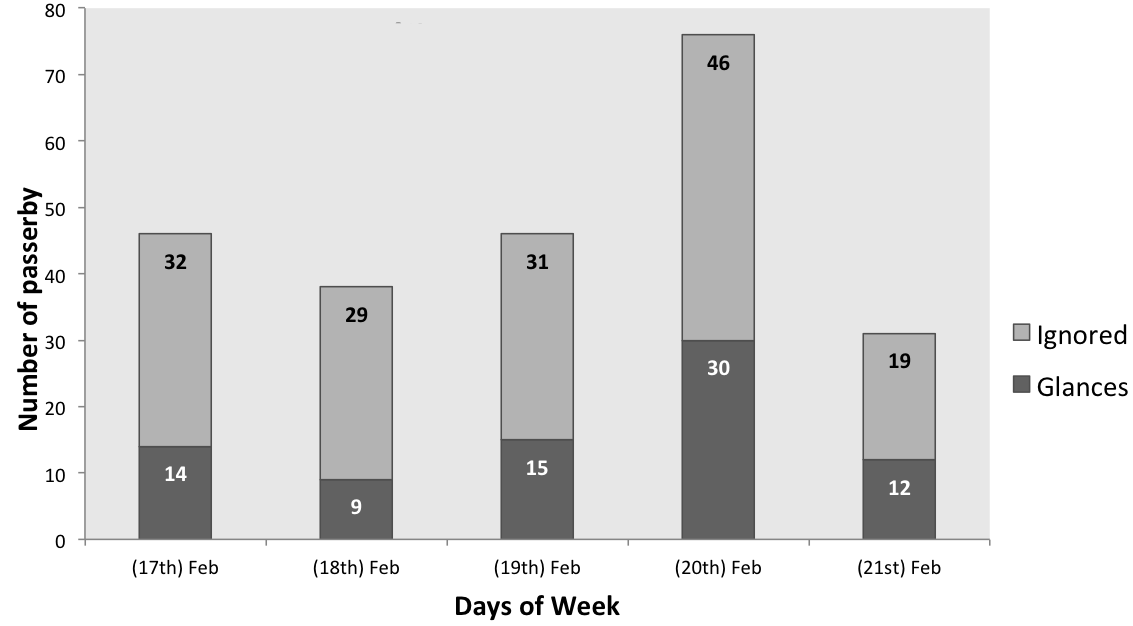
\includegraphics[width=110mm,height=60mm]{Figures/8/mobile_inter_findings/mobile_Inter_chart}%
    \caption{Mobile interactive attention level chart}%
    \label{fig:mobileattentionlevelchart}%
\end{figure}


\begin{figure}[H]
    \centering
    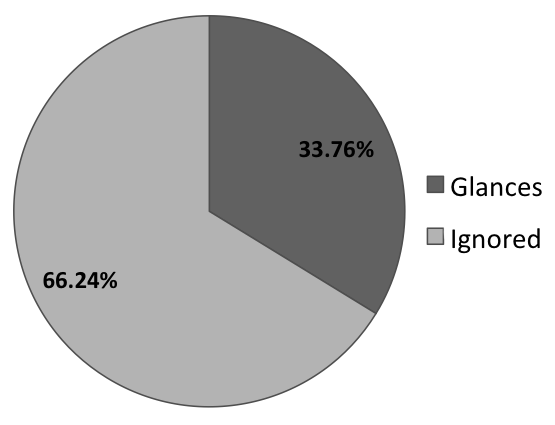
\includegraphics[width=110mm,height=60mm]{Figures/8/mobile_inter_findings/mobile_inter_percentage}
    \caption{Mobile interactive Attention level percentage}%
    \label{fig:bodyattentionlevelpercentage}%
\end{figure}


\item Engagement time

In average the engagement for the passerby took 21.70 seconds

\item Passerby and interactions


\begin{figure}[H]
    \centering
    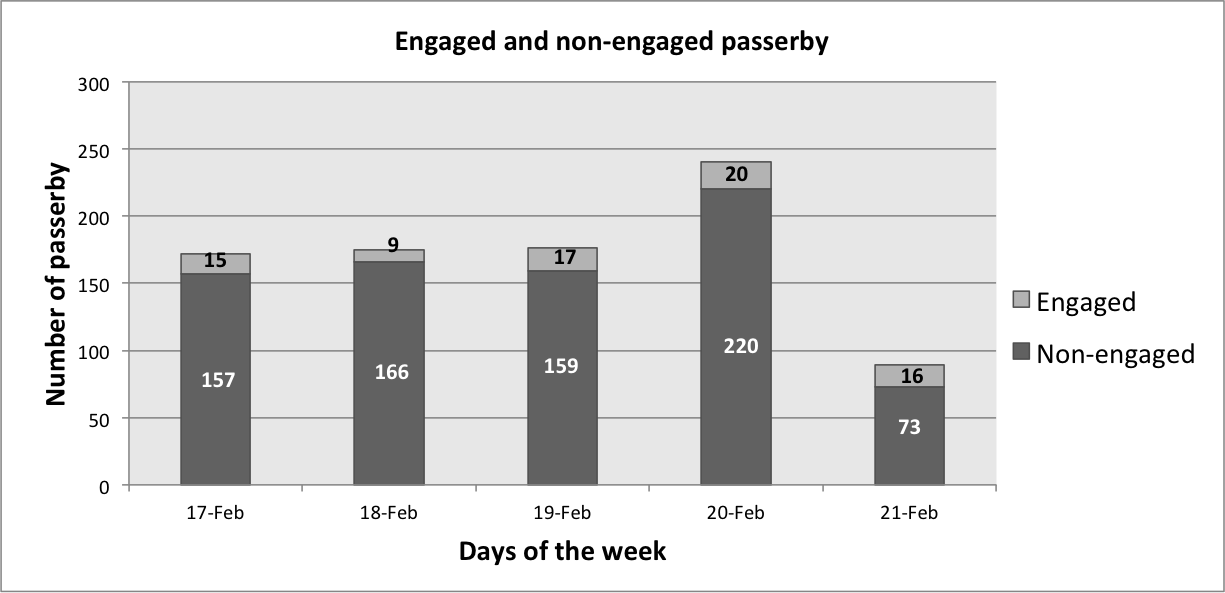
\includegraphics[width=110mm,height=60mm]{Figures/8/mobile_inter_findings/mobile_inter_engage_day}
    \caption{Mobile interactive Number of engaged passerby}%
    \label{fig:mobileengagedandengagedby}%
\end{figure}

\begin{figure}[H]
    \centering
    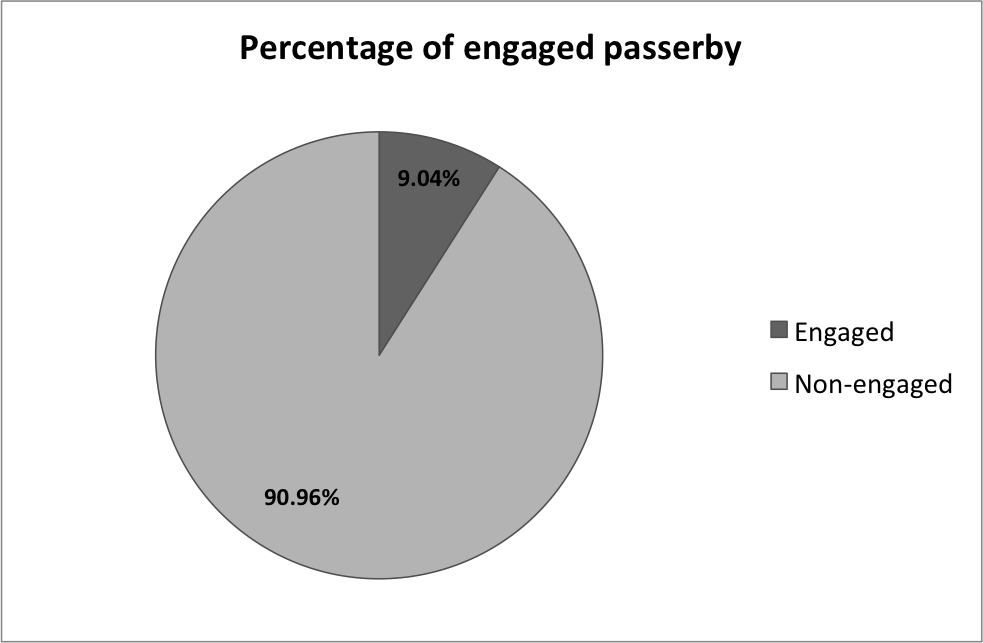
\includegraphics[width=110mm,height=60mm]{Figures/8/mobile_inter_findings/mobile_eng_percentage}
    \caption{Mobile interactive percentage of engaged passerby}%
    \label{fig:mobileengagedpasserbypercentage}%
\end{figure}

\item Landing and Honeypot effects

\begin{table}[H]
\caption{Mobile Interactive Landing and honeypot effect}
\label{tab:landingandhonypot_mobile}
\centering
\begin{tabular}{| l | c | c |}
\toprule
\tabhead{Days} & \tabhead{Landing effect} & \tabhead{Honeypot effect} \\
\midrule
\textbf{17 Feb}  & 0 &  1 \\
\textbf{18 Feb}  & 1 &  0 \\
\textbf{19 Feb}  & 2 &  0 \\
\textbf{20 Feb}  & 0 &  0 \\
\textbf{21 Feb}  & 1 &  1 \\
\bottomrule
\end{tabular}
\end{table}



\item Interview


\hilight{complete the interview report}



\item Note taking


see Appendix \ref{AppendixD}.11


\item Other observations

\end{enumerate}



\subsection{Comparison of advertisements}

\subsubsection {Number of passerby}
Because the advertisements techniques were not conducted in the same days, which could ruin comparison because of different number of passers-by everyday and each week, there was a need to first compare the number of passers-by and prove that they were not statistically different in between. \\

\textbf{Hypothesis: }
\begin{itemize}
\item \textbf{H0:} There was no difference between numbers of passerby of each week.
\item \textbf{H1:} There was a difference between numbers of passerby of each week.
\end{itemize}

The bellow is the table of passerby for three weeks.

\begin{table}[H]
\caption{Number of passerby in three weeks}
\label{tab:passerbyofthreeweeks}
\centering
\begin{tabular}{| l | c | c | c |}
\toprule
\tabhead{Days} & \tabhead{First week} & \tabhead{Second week} & \tabhead{Third week} \\
\midrule
\textbf{Day 1}  & 232 & 178 &  172 \\
\midrule
\textbf{Day 2}  & 170 & 220 &  175 \\
\midrule
\textbf{Day 3}  & 212 & 259 &  176 \\
\midrule
\textbf{Day 4}  & 209 & 216 &  240 \\
\midrule
\textbf{Day 5}  & 208 & 122 &  89  \\
\midrule
\textbf{Total}  & 1031 & 995 & 852 \\
\bottomrule
\end{tabular}
\end{table}

ANOVA test revealed that there is no significant different of passers-by between each of the weeks.
 \emph{(F2,5)=0.8873, p >.05 (p=0.437)}
 So based on this the \emph{H0} hypothesis is being accepted and \emph{H1} hypothesis is being rejected. This gives us confidence to proceed our comparisons.




\subsubsection {Attention Level Comparison}

As can be seen Non-interactive (first week) had \%28.83 number of glances, the Body-interaction (second week) had almost \%10 high number of glances (\%38.70) than non-interactive, The mobile Interaction had higher glances (\%33.75) from non-interactive but still less than body interaction. But with this we can not conclude that body interaction had higher until we statistically state them.

To compare which of the the three methods drove more passers-by attention, the data of number of glances for each of the weeks are gathered as bellow and first we want to find out if these data are statistically different or not.\\

\textbf{Hypothesis: }
\begin{itemize}
\item \textbf{H0:} There was no difference between numbers of passerby of each week.
\item \textbf{H1:} There was a difference between numbers of passerby of each week.
\end{itemize}



% table
\begin{table}[H]
\caption{Cross tabulation for each week attention level }
\label{tab:crosstabulationweeks}
\centering
\begin{tabular}{| l | c | c | c |}
\toprule
\tabhead{Method} & \tabhead{Glanced (\%)} & \tabhead{Ignored} & \tabhead{Total } \\
\midrule
\textbf{First week}     & 111(\%28.83)   &   274      &   385\\
\midrule
\textbf{Second week }   & 96 (\%38.70)   &   152      &   248\\
\midrule
\textbf{Third week }    & 80 (\%33.75)   &   157      &   237\\
\midrule
\textbf{Total }         & 287            &   583      &   870\\
\bottomrule
\end{tabular}
\end{table}



Running Chi-squared test to see the significant between different advertisement conditions and the bellow result shows that they are statistically significant.
${\chi}^2$\emph{(2, N=870)=6.7452, p < .05 (p=.03431)}, so \emph{H0} is rejected and \emph{H1} hypothesis would be accepted.
To find the actual difference, each pairs were tested in between using again Chi-squared test.

\begin{enumerate}
\item Non-Interactive Vs Body Interactive \\
The finding shows that body interactive advertisement had had significant number of glances than non-interactive advertisement. \\
${\chi}^2$\emph{(1, N=633)=6.6883, p < .05 (p=.0097)}

\item Non-Interactive Vs Mobile Interactive  \\
The finding suggests that there is no significant difference between them.\\
${\chi}^2$\emph{(1, N=622)=1.6716, p < .05 (p=.196039)}

\item Body interactive Vs Mobile Interactive \\
As can be expected the glances are not statistically significant among the body and mobile interactive advertisement.\\
${\chi}^2$\emph{(1, N=485)=1.2866 , p < .05 (p=.25667)}

\end{enumerate}


\subsubsection {Engaged and Non-engaged passerby}
This test is to find out if there is a difference between number of Engaged passerby or not between the weeks.

\textbf{Hypothesis: }
\begin{itemize}
\item \textbf{H0:} There is no difference between the numbers of Engaged passerby between the weeks.
\item \textbf{H1:} There is a difference between the numbers of Engaged passerby between in each weeks.
\end{itemize}

The bellow table lists all number of engaged and non-engaged passers-by for three weeks.


\begin{table}[H]
\caption{Number of engaged passerby in three weeks}
\label{tab:engagedofthreeweeks}
\centering
\begin{tabular}{| l | c | c | c |}
\toprule
\tabhead{Days} & \tabhead{First week} & \tabhead{Second week} & \tabhead{Third week} \\
\midrule
\textbf{Day 1}  & 16 & 25 &  15 \\
\midrule
\textbf{Day 2}  & 18 & 21 &  9 \\
\midrule
\textbf{Day 3}  & 15 & 26 &  17 \\
\midrule
\textbf{Day 4}  & 15 & 20 &  20 \\
\midrule
\textbf{Day 5}  & 15 & 23 &  16  \\
\midrule
\textbf{Total}  & 79 & 115 & 77 \\
\bottomrule
\end{tabular}
\end{table}

The ANOVA test strongly suggests that there is a significant difference of the number of Engaged passersby between these three weeks.\\
 \emph{(F2,5)=11.20, p >.05 (p=.002)}

To find where are the main difference between them, the Post-Hoc Tukey’s HSD test was conducted on each three pairs of the week to point out which of them exhibit statistically significant difference. 


\begin{table}[H]
\caption{Post-Hoc Tukey’s HSD}
\label{tab:engage-non-posthoctukey}
\centering
\resizebox{\textwidth}{!}{ 
\begin{tabular}{| l | c | c | c |}
\toprule
\tabhead{Methods} & \tabhead{Tukey HSD Q statistic} & \tabhead{Tukey HSD p-value} & \tabhead{Tukey HSD inferfence} \\
\midrule
\textbf{A vs B}  & 5.6337 & 0.0047509 & \cellcolor{green!80} ** p<0.01  \\
\midrule
\textbf{A vs C}  & 0.3130 & 0.8999947 &  \cellcolor{red!80} insignificant \\
\midrule
\textbf{B vs C}  & 5.9467 & 0.0032197 & \cellcolor{green!80} ** p<0.01 \\

\bottomrule
\end{tabular}
}
\end{table}


Method A, B and C refers to (Non-interactive, body interactive and mobile interactive) advertisement accordingly. As can be seen from the above chart, there is no significant difference between group A and C and group B which is body interactive advertisement shows a significant difference between A and C. it shows that the body interactive advertisement engaged significantly more passersby than other two types of advertisement.


\subsubsection {Landing effect}
The bellow table shows how many landing effects were recorded from the depth observation video for each of the weeks.\\


\textbf{Hypothesis: }
\begin{itemize}
\item \textbf{H0:} There is no difference between the numbers of Engaged passerby between in each week.
\item \textbf{H1:} There is a difference between the numbers of Engaged passerby between in each week.
\end{itemize}

\begin{table}[H]
\caption{Number of Landing effects in three weeks}
\label{tab:landingeffectthreeweeks}
\centering
\begin{tabular}{| l | c | c | c |}
\toprule
\tabhead{Days} & \tabhead{First week} & \tabhead{Second week} & \tabhead{Third week} \\
\midrule
\textbf{Day 1}  & 1 & 2 &  0 \\
\midrule
\textbf{Day 2}  & 0 & 3 &  1 \\
\midrule
\textbf{Day 3}  & 2 & 2 &  2 \\
\midrule
\textbf{Day 4}  & 0 & 2 &  0 \\
\midrule
\textbf{Day 5}  & 1 & 3 &  1  \\
\bottomrule
\end{tabular}
\end{table}

ANOVA test reveals that there is a significant difference between one or two above conditions, ( \emph{(F2,5)=7.529, p >.05 (p=.008)}). So we reject the Null hypothesis and state that one of the above conditions are statistically significant from the others, to confirm this we again run Post-Hoc Tukey’s HSD test on the above data.


\begin{table}[H]
\caption{Post-Hoc Tukey’s HSD results}
\label{tab:landing-non-posthoctukey}
\centering
\resizebox{\textwidth}{!}{ 
\begin{tabular}{| l | c | c | c |}
\toprule
\tabhead{Methods} & \tabhead{Tukey HSD Q statistic} & \tabhead{Tukey HSD p-value} & \tabhead{Tukey HSD inferfence} \\
\midrule
\textbf{A vs B}  & 4.7527 & 0.0144554 & \cellcolor{green!50} * p<0.05  \\
\midrule
\textbf{A vs C}  & 0.0000 & 0.8999947 &  \cellcolor{red!80} insignificant \\
\midrule
\textbf{B vs C}  & 5.9467 & 0.0144554 & \cellcolor{green!50} * p<0.05 \\

\bottomrule
\end{tabular}
}
\end{table}


Group A, B and C refers to (Non-interactive,body interactive and mobile interactive) advertisement accordingly As can be seen the test shows that the condition A and C are insignificant but condition B is significant from A and C, which means that body interactive advertisement has statistically higher landing effects than other 


\subsubsection {Honeypot effect}
The bellow table shows how many honeypot effects were recorded from the depth observation video.\\

\textbf{Hypothesis: }
\begin{itemize}
\item \textbf{H0:} There is no significant difference between the numbers of honeypot effect for the above three advertisement types.
\item \textbf{H1:} There is significant difference between the numbers of honeypot effect for the above three advertisement types.
\end{itemize}


\begin{table}[H]
\caption{Number of Honeypot effect in three weeks}
\label{tab:landingeffectthreeweeks}
\centering
\begin{tabular}{| l | c | c | c |}
\toprule
\tabhead{Days} & \tabhead{First week} & \tabhead{Second week} & \tabhead{Third week} \\
\midrule
\textbf{Day 1}  & 1 & 2 &  1 \\
\midrule
\textbf{Day 2}  & 1 & 3 &  0 \\
\midrule
\textbf{Day 3}  & 2 & 2 &  0 \\
\midrule
\textbf{Day 4}  & 2 & 5 &  0 \\
\midrule
\textbf{Day 5}  & 1 & 3 &  1  \\
\bottomrule
\end{tabular}
\end{table}


ANOVA test reveals that there is a significant different between the groups
(\emph{(F2,5)=12.29, p >.05 (p=.001)}), and after doing Post-hoc Tukey test it revealed that there is significant difference of Honeypot between Body Interactive and Mobile interactive advertisement, but less statistical different between Non-interactive and body interactive as the online tool gave one star for A and B and two stars for B and C.



\begin{table}[H]
\caption{Post-Hoc Tukey’s HSD results}
\label{tab:honeypot-non-posthoctukey}
\centering
\resizebox{\textwidth}{!}{ 
\begin{tabular}{| l | c | c | c |}
\toprule
\tabhead{Methods} & \tabhead{Tukey HSD Q statistic} & \tabhead{Tukey HSD p-value} & \tabhead{Tukey HSD inferfence} \\
\midrule
\textbf{A vs B}  & 4.2762 & 0.0264780 & \cellcolor{green!50} * p<0.05  \\
\midrule
\textbf{A vs C}  & 2.6726 & 0.1836687 &  \cellcolor{red!80} insignificant \\
\midrule
\textbf{B vs C}  & 6.9488 & 0.0010053 & \cellcolor{green!100} ** p<0.01 \\
\bottomrule
\end{tabular}
}
\end{table}

























































